\documentclass[../../main.tex]{subfiles}

\begin{document}
En este apéndice se describe en detalle todo el proceso para poder manejar la aplicación por cualquier usuario.  \\

Esta aplicación ofrece dos funcionalidades:
\begin{enumerate}
    \item Extraer información de la red social usando la \gls{ipa}.
    \item Trabajar con los datos guardados en la base de datos.
\end{enumerate}

Estas dos opciones vienen separadas en el menú superior de la aplicación, la cual la primera opción se corresponde con \textit{Data Extraction} y la segunda opción con \textit{\Gls{reddit}}.

\subsection{Extracción de datos}

Para este apartado pinchamos en el menú en \textit{Data Extraction \textrightarrow  \Gls{reddit}}, una vez pinchado en este enlace en el apartado izquierdo aparecerá una barra lateral con campos a modificar como el siguiente:

\begin{figure}[H]
\centering
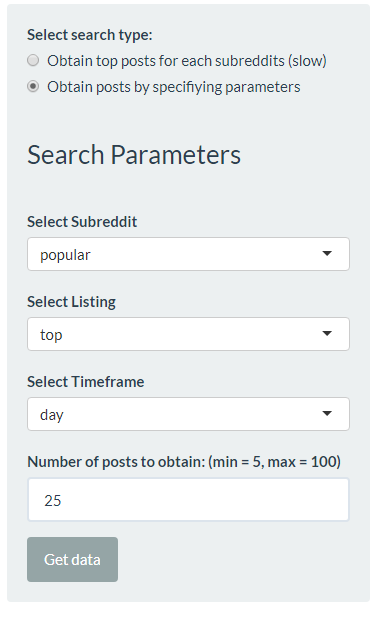
\includegraphics[height=250pt]{images/apendices/data-extract1.1.png}
\caption{Aplicación \Gls{shiny} - Barra lateral de la Opción 1 del apartado Extracción de los datos}
\end{figure}

En esta pantalla viene seleccionado por defecto la opción \textit{Obtain posts by specifying parameters}, esta opción nos permite obtener un número de publicaciones de un \gls{subreddit} en concreto o de una etiqueta llamada popular donde engloba las publicaciones con mas controversia en este momento.

Con esta opción seleccionada es posible seleccionar los siguientes campos:
\begin{itemize}
    \item \textbf{Select \Gls{subreddit}}. Permite indicar el \gls{subreddit} del cual obtener las publicaciones. Por defecto, viene marcada la opción \textit{popular} pero es posible especificar un subreddit en concreto. 
    \item \textbf{Select Listing}. Permite especificar en qué orden se buscan las publicaciones. Por defecto, viene marcada la opción \textit{top} pero es posible especificar otro tipos de ordenes como \textit{new} o \textit{rising}.
    \item \textbf{Select Timeframe}. Permite especificar el plazo de tiempo en el cual se deben obtener las publicaciones. Por defecto, viene marcada la opción \textit{día} pero es posible seleccionar otros plazos como pueden ser la \textit{hora}, \textit{semana}, \textit{mes}, \textit{año} o \textit{todos}.
    \item \textbf{Number of posts to obtain}. Permite especificar el número de publicaciones a obtener. Por defecto, viene establecido 25 publicaciones el cual es un número razonable ya que suele tardar unos 30 segundos en ejecutarse, cuanto más alto sea este valor más tarda la operación en finalizar.
\end{itemize}

Si se selecciona la otra opción disponible \textit{Obtain top posts for each subreddit} se obtiene una barra lateral con unas opciones similares a la opción anterior

\begin{figure}[H]
\centering
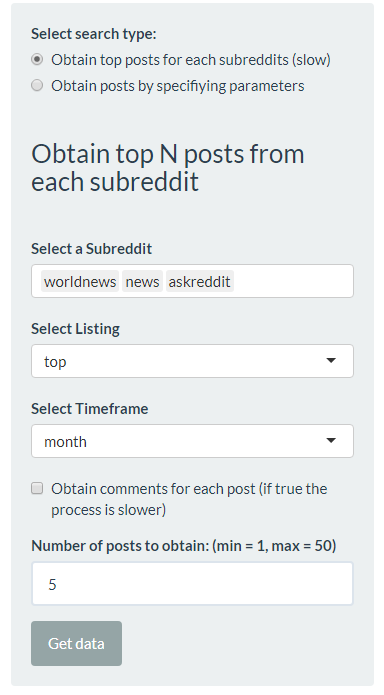
\includegraphics[height=250pt]{images/apendices/data-extract2.1.png}
\caption{Aplicación \Gls{shiny} - Barra lateral de la Opción 2 del apartado Extracción de los datos}
\end{figure}

Con esta opción es posible establecer los siguientes campos:
\begin{itemize}
    \item \textbf{Select \Gls{subreddit}}. Permite indicar el \gls{subreddit} o \glspl{subreddit} del cual obtener las publicaciones, también existe la opción para seleccionar todos los subreddits. Por defecto, viene marcada la opción \textit{worldnews}, \textit{news} y \textit{askreddit} pero es posible añadir o quitar elementos de esta lista. 
    \item \textbf{Select Listing}. Permite especificar en qué orden se buscan las publicaciones. Por defecto, viene marcada la opción \textit{top} pero es posible especificar otro tipos de ordenes como \textit{new} o \textit{rising}.
    \item \textbf{Select Timeframe}. Permite especificar el plazo de tiempo en el cual se deben obtener las publicaciones. Por defecto, viene marcada la opción \textit{día} pero es posible seleccionar otros plazos como pueden ser la \textit{hora}, \textit{semana}, \textit{mes}, \textit{año} o \textit{todos}.
    \item \textbf{Obtain comments for each post}. Permite especificar si obtiene los comentarios de cada publicación. Si se activa esta opción el proceso de obtención de los datos es más lento.
    \item \textbf{Number of posts to obtain}. Permite especificar el número de publicaciones a obtener. Por defecto, viene establecido 25 publicaciones el cual es un número razonable ya que suele tardar unos 30 segundos en ejecutarse, cuanto más alto sea este valor más tarda la operación en finalizar.
\end{itemize}

Una vez seleccionado los valores deseados en ambos casos se pincha en el botón \textit{Get data} y a la derecha de la barra lateral aparecerá el resultado obtenido.  \\

Este resultado se divide en dos apartados, uno mostrando el resultado obtenido y el tipo de dato de cada columna, y otro apartado donde se muestra una tabla donde se puede visualizar de forma más amigable al usuario los datos.

\subsection{Trabajo con los datos}


Para este apartado pinchamos en el menú en \textit{\Gls{reddit}}, una vez pinchado en este menú tenemos tres opciones disponibles \textit{Posts}, \textit{Awards} y \textit{Comments}. Para cada opción se muestra una barra lateral como el siguiente:

\begin{figure}[H]
\centering
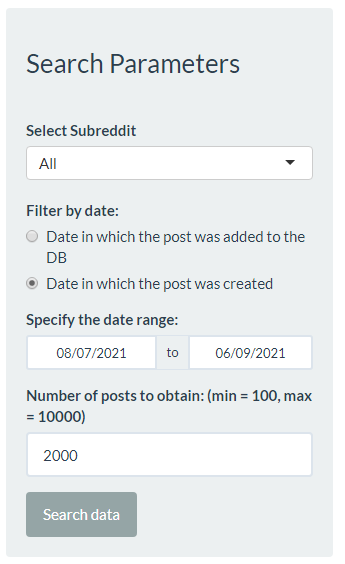
\includegraphics[height=250pt]{images/apendices/db-sidebar.png}
\caption{Aplicación \Gls{shiny} - Barra lateral del apartado Análisis de los datos}
\end{figure}

En el caso de \textit{Awards} y \textit{Comments} aparece un selector para seleccionar qué orden se debe aplicar para recoger los datos de la base de datos.


En esta barra lateral es posible establecer los siguientes campos:
\begin{itemize}
    \item \textbf{Select \Gls{subreddit}}. Permite indicar el \gls{subreddit} del cual obtener las publicaciones. Por defecto, viene marcada la opción \textit{popular} pero es posible especificar un subreddit en concreto. Esta opción solo esta visible en el apartado de \textit{Posts}.
    \item \textbf{Select Order}. Permite indicar en qué orden se recogen los datos del servidor. Esta opción solo está visible en los apartados \textit{Awards} y \textit{Comments}.
    \begin{figure}[H]
    \centering
    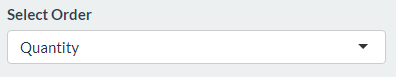
\includegraphics[height=40pt]{images/apendices/db-sidebar2.png}
    \caption{Aplicación \Gls{shiny} - Selector de Orden}
    \end{figure}
    \item \textbf{Filter by date}. Permite especificar si se obtiene las publicaciones ordenadas por su fecha de creación o fecha en la que se insertó en el servidor de base de datos.
    \item \textbf{Specify the date range}. Permite especificar en qué rango de fechas se deben obtener los registros. Por defecto, viene establecido como fecha de fin la fecha actual y fecha de inicio 60 días anteriores a la fecha actual.
    \item \textbf{Number of posts to obtain}. Permite especificar el número de publicaciones a obtener. 
\end{itemize}

Una vez seleccionado los valores deseados en ambos casos se pincha en el botón \textit{Get data} y a la derecha de la barra lateral aparecerá el resultado obtenido.  \\

En el resultado obtenido aparecerá un sub menú como aparece en la siguiente imagen:

\begin{figure}[H]
\centering
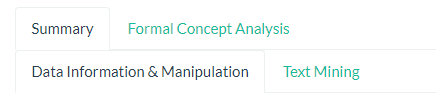
\includegraphics[height=60pt]{images/apendices/db-menu.png}
\caption{Aplicación \Gls{shiny} - Sub Menú del apartado de Análisis de los datos}
\end{figure}

\subsubsection{Resumen}

En la pestaña \textit{Data Information \& Manipulation} obtenemos diversa información sobre los datos obtenidos del servidor de base de datos.  \\

En esta misma pantalla se ofrece la posibilidad de descargar la matriz binaria completa en un fichero \gls{csv} mediante el botón:

\begin{figure}[H]
\centering

\includegraphics[height=30pt]{images/apendices/db-data-dwnld.png}
\caption{Aplicación \Gls{shiny} - Descargar matriz binaria}
\end{figure}

En la pestaña \textit{Text Mining} se obtiene más información sobre los términos que aparecen en las publicaciones.

\subsubsection{Análisis de Conceptos Formales}

En este apartado del sub menú se divide en cuatros sub apartados tales como aparece en la siguiente imagen:

\begin{figure}[H]
\centering
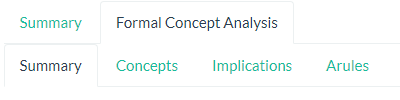
\includegraphics[height=50pt]{images/apendices/db-fca-menu.png}
\caption{Aplicación \Gls{shiny} - Sub Menú del apartado de Análisis de Conceptos Formales}
\end{figure}

En la pestaña \textit{Summary} se muestra información sobre el número de transacciones que hay en el conjunto de datos y a partir de las reglas no redundantes crea el contexto formal.  \\

En este misma pantalla se ofrece la posibilidad de descargar el contexto formal en \gls{latex} mediante el botón:

\begin{figure}[H]
\centering

\includegraphics[height=30pt]{images/apendices/db-fca-latex.png}
\caption{Aplicación \Gls{shiny} - Descargar en \gls{latex}}
\end{figure}

En la pestaña \textit{Concepts} se obtienen los conceptos para el contexto formal y se trabaja sobre estos conceptos calculados.  \\

En la pestaña \textit{Implications} se calculan las implicaciones para el contexto formal y se trabaja sobre estas, en la cual se intenta realizar una recomendación.  \\

En la pestaña \textit{Arules} se exporta las implicaciones a reglas de asociación y se muestra por pantalla diversas gráficas en las cuales se visualizan las reglas no redundantes y las reglas significantes, así mismo se ordenan las reglas por las propiedades \textit{\gls{lift}} y \textit{\gls{support}} para su posterior visualización.  \\

\end{document}